% This is samplepaper.tex, a sample chapter demonstrating the
% LLNCS macro package for Springer Computer Science proceedings;
% Version 2.20 of 2017/10/04
%
\documentclass[runningheads]{llncs}
%
\usepackage{graphicx}
\usepackage{caption}
\usepackage{subfigure}
% Used for displaying a sample figure. If possible, figure files should
% be included in EPS format.
%
% If you use the hyperref package, please uncomment the following line
% to display URLs in blue roman font according to Springer's eBook style:
% \renewcommand\UrlFont{\color{blue}\rmfamily}

\begin{document}
%
\title{Optimizing the computational efficiency of 3D segmentation models for connectomics}

\author{
First Author\inst{1}\orcidID{0000-1111-2222-3333} 
\and
Second Author\inst{2,3}\orcidID{1111-2222-3333-4444} 
\and
Third Author\inst{3}\orcidID{2222--3333-4444-5555}
}
%\author{
%Weihao Zhuang  \inst{1} %\orcidID{0000-1111-2222-3333} 
%\and
%Hascoet Tristan \inst{1} %\orcidID{1111-2222-3333-4444} 
%\and
%Takashima Ryoichi \inst{1}
%\and
%Takiguchi Tetsuya \inst{1}
%\authorrunning{F. Author et al.}
%}

% First names are abbreviated in the running head.

% If there are more than two authors, 'et al.' is used.

%
%
%\institute{Kobe university
%
%%\email{lncs@springer.com}\\
%
%%\url{http://www.springer.com/gp/computer-science/lncs} \and
%
%%ABC Institute, Rupert-Karls-University Heidelberg, Heidelberg, Germany\\
%
%%\email{\{abc,lncs\}@uni-heidelberg.de}
%
%}
%
%%
%
%\maketitle              % typeset the header of the contribution
%
%%
%
%\begin{abstract}
%
%The field of connectomics aims to map the interconnections between biological neurons within nervous systems at the scale of single synapses to gain insights into the structure and functional organization of biological neural networks. A critical task for the success of the connectomics enterprise is the segmentation of neurites from high precision electron microscopy (EM) images. This task requires models to be both accurate and computationally efficient in order to process large volumes of very high precision microscopy images. In recent years, segmentation models have become very accurate. In this paper, we analyse the computational efficiency of one such successful 3D U-Net and identify several computational bottlenecks. We propose different optimizations to increase the computational efficiency of this model and achieve a x% speed up with minimal accuracy loss.
%
%
%
%\keywords{Neurite segmentation  \and 3D CNN \and Computational efficiency}
%
%\end{abstract}
%
%%
%
%\section{Introduction}
%
%Precise reconstruction of neural connectivity is of great importance to understand the functional organization of biological nervous systems. 3D electron microscopy (EM) can capture large volume of neuronal tissues within nano-scale precision, which allows for the identification of even the smallest neuronal objects like vesicles. With advances in imaging technologies, EM systems can now produce terabytes of images within hours. Manually annotating each of the neurons within such large EM volumes is simply impractical as it would requires lifetimes of manual labeling from highly skilled experts to segment. Hence, high-precision segmentation models are needed to automate the reconstruction of neuronal circuits. 
%
%
%
%Current state-of-the art models for 3D neurite segmentation proceeds in three steps, as illustrated in Figure 1. First, a CNN is trained to detect boundaries between neurons in the raw EM images. In a second step, over-segmentation maps are computed from the boundary map. This is typically done by non-parametric algorithms like Watershed. Finally, an agglomeration algorithm is used to process the over-segmented results typically produced by the Watershed algorithm. 
%
%
%
%In this pipeline, the first step is the computational bottleneck as both the training of the segmentation model and the inference using trained model are computationally expensive. The benefits of optimizing the computational efficiency of the 3D U-Net is two-folds: 
%
%
%
%First, computationally efficient models would significantly ease the inference step: AS the resolution needed to accurately detect synaptic connections is on the order of a few nanometers, only a cubic millimeter of brain tissue at this resolution represents on the order of X Bytes. Processing such a large volume is considerable computational challenge. Hence optimized computations will be needed in order to enable the processing of large brain volumes.
%
%
%
%However, the most impactful benefit concerns the training step: As training an unoptimized model takes up to days on a single GPU machine, the iterative process needed to fine-tune models and experiment with different architectures and loss functions is very slow. Optimizing the computational efficiency of our model would enable us to more efficiently explore the space of solution. Getting faster iteration cycles would allow us to more efficiently come up with better solutions. 
%
%
%
%In this paper, we thus analyse the computational efficiency of a successful 3D U-Net segmentation model. We identify several factors responsible for slowing down the computations. We propose several tweaks to speed up the computations and obtain a relative speed up of X%. Many optimizations remain to be done. 
%
%
%
%In the next section, we start by presenting related research. We then analyze the baseline model in Section XXX, and present our optimization in Section XXX. Section XXX discusses the results of our experiments.
%
%
%
%
%
%\section{Baseline model Analysis}
%
%
%
%\subsection{Baseline model}
%
%%3dunet config
%
%%\subsection{Background knowledge}
%
%%Reason of need for profile neural network.
%
%We start by analyzing the computational efficiency of our baseline model.
%
%We chose the 3D U-Net proposed by X et al \cite{}, as illustrated in Figure 3, 
%
%which was the first work to surpass human accuracy on the SNEMI3D neurite segmentation challenge.
%
%We only adapt their architecture to fit the anisotropy of our own dataset by replacing the 
%
%2D pooling operations of the first two layers by 3D pooling operations.
%
%
%
%
%
%\subsection{Model analysis}
%
%
%
%\begin{figure}[p]
%
%\centering
%
%
%
%  \begin{minipage}{7cm}
%
%  \centering     
%
%  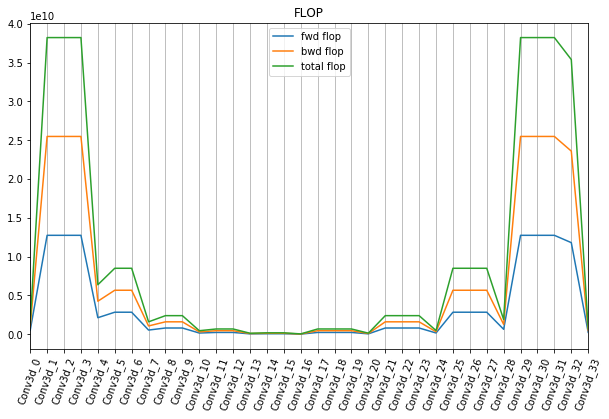
\includegraphics[scale=0.42]{FLOP.png}   
%
%  \end{minipage}
%
%
%
%\caption{3D Unet profile results} 
%
%\label{fig:1} 
%
%\end{figure}
%
%
%
%
%
%%Factors effect computation efficiency.
%
%%What is FLOP, FLOPs, A.I., MAC
%
%%profile factors
%
%Figure X analyzes the processing time spent in each layer of the network.
%
%
%
%The time ($s$) $t(l)$ required by a given layer $l$ to process an input batch can be 
%
%decomposed into the number of operations (FLOP) $O(l)$ divided by the computational efficiency (FLOP/s) $E(l)$ of the layer:
%
%
%
%$$t(l) = 0(l) / E(l) $$
%
%
%
%The total processing time T required by the model $M$ to process an input batch is the sum 
%
%of the time needed by each layer:
%
%
%
%$$T = \sum_{l \in M} t(l)$$
%
%
%
%Figure XXX shows the number of operations of, the efficiency, and the processing time spent in each layer of the baseline model 
%
%in the order of their processing: the left-most value of each plot represents the input layer, 
%
%followed by the next lower layer, up until the output layer represented by the right-most value of the plot.
%
%In reality, batch normalization, ReLU, pooling and skip connections should be represented on these plots between each convolution.
%
%However, as the computations are dominated by convolution layers, we consider these layers negligible
%
%and only show the analysis of convolutions for readability. 
%
%
%
%\section{Baseline Model Optimization}
%
%%After the analysis, how to optimize.
%
%%Profile results analysis.
%
%We minimize the total processing time $T$ by optimizing individual layers.
%
%For a given layer $l$, minimizing the processing time $ t(l) $ can be achieved in two ways:
%
%We can either reduce the number of operations $O(l)$ of a given layer $l$, or increase its efficiency $E(l)$ 
%
%Reducing the number of operations $O(l)$ is done by modifying the architecture parameters, 
%
%which we explain in the following section.
%
%Increasing the computational efficiency is done by optimizing the low-level implementation of the convolutions,
%
%which we explain in Section XXX.
%
%
%
%\subsection{Architectural optimization}
%
%
%
%Figure XXX compares the distribution of FLOP among each layers of a 2D ResNet \cite{} and our baseline 3D UNet.
%
%The 2D-ResNet computations are evenly distributed among its layers, while the 3D UNet computations concentrate on the 
%
%first and last layers of the network, which consume XXX \% of the computational budget.
%
%Intuitively, this seems misguided as there is no rational for the low level feature processing to be that much more computationally 
%
%expensive than the higher level feature processing.
%
%
%
%The 2D ResNet has been carefully parameterized so as to maintain a constant computational 
%
%for convolutional layers across the full model:
%
%In ResNets, the number of channels is doubled after each pooling layers, 
%
%while pooling reduce each spatial dimension by a factor of 2.
%
%
%
%The computational complexity (FLOP) of a convolution operation with stride 1 at layer $l$ is given by:
%
%
%
%$$ O(l) = h \times w \times c^2 \times bs  \times kh  \times kw $$
%
%
%
%Where $h,w$ represents the input image dimensions, 
%
%the input and output channels $c$ are considered equal, 
%
%and $kh,kw$ represent the spatial dimensions of the kernel.
%
%
%
%Hence, the computational complexity is quadratic in both the input spatial dimension ($h \times w$),
%
%and the channel dimension ($c^2$).
%
%Denoting by $l'$ an upstream layer of $l$ after pooling, the computational complexity in ResNet parameterization is given by:
%
%
%
%$$ O(l') = h' \times w' \times c'^2 \times bs'  \times kh'  \times kw' $$
%
%$$ O(l') = (h/2) \times (w/2) \times (c \times 2)^2 \times bs  \times kh  \times kw $$
%
%$$ O(l') = h \times w \times c^2 \times bs  \times kh  \times kw $$
%
%$$ O(l') = O(l) $$
%
%
%
%Hence, by doubling the number of channels after each pooling operations, ResNet maintains a computational cost constant with depth.
%
%
%
%To maintain a constant computational cost with depth, 3D CNNs should thus scale the channel dimension
%
%by a factor of $\sqrt{8}$ after each pooling operation, 
%
%which is far more than the scaling factor used by our baseline model.
%
%This explains why the computational cost is concentrated in the first layers as 
%
%it is exponentially decreased with depth.
%
%
%
%To further reduce the computational cost of the first and last layer, 
%
%we draw inspiration from efficient ResNet implementations and replace the first and
%
%Last layer of our model by strided and fractionally strided convolutions respectively.
%
%This allows us to minimize the amount of computation performed at full resolution.
%
%
%
%\subsection{Implementation optimization}
%
%
%
%The following figure shows the profile result of training a 3D UNet. 
%
%%first layer takes the most time.
%
%From the figure (a) and figure (c), we can observe that 3D UNet first few layers and last few layers spend the most time on training due to their high FLOP. 
%
%However, those layer are used to extract low features. It is inefficient to spend a lot of time extracting low features.
%
%
%
%%Cannot reach the maximum theoretical computational efficiency
%
%According to figure (b), current maximum computational efficiency is close to that of 1.6TFLOPs, but our experimental equipment: Nvidia TITAN X, can reach 11TFLOPs in theory. If each layer of the model can maximize the computational efficiency, we can speed up at least 10 times. 
%
%
%
%%compare to ResNet
%
%
%
%
%
%%reduce FLOP
%
%Since computation time can be obtained by FLOP divided by computational efficiency, we optimize our model in two ways. One, reduce FLOP appropriately. Another, make schedule of computation and data transfer more efficient.
%
%
%
%%use stride convolution
%
%We use stride convolution to optimize first layer that can reduce the shape of the output and FLOP since the linear relationship between FLOP and shape of output.
%
%
%
%%use tvm to optimize computation, distange of cudnn, what is tvm, halide, autotvm 
%
%For optimize computation schedule, usually, cuDNN[?] is the first choice of most researchers. cuDNN is a handwritten low-level deep learning implement acceleration library, provided by NVIDIA for its GPUs. However it is closed source. MKL-DNN, a deep learning acceleration library was proposed by Intel for their CPU running deep learning applications. 
%
%%disadvantages of cudnn
%
%Both cuDNN and MKL-DNN are optimized for specialized hardware. It is time-consuming for manual hardware optimization for different device or deep learning operation without using excited deep learning acceleration libraries.
%
%
%
%%Halide and tvm introduction
%
%Halide[?], a programming language which main innvation is computation/schedule separation that allow us design different schedule for different devices. TVM[?] extend the idea of Halide, which not only separates computation from schedule, but also uses machine learning to search efficient schedule implements which can towards peak hardware performance in a large optimization search space (memory tiling, parallelization, loop transformations, vectorization, tensorization, etc).
%
%%we choose tvm as a low-level code general tool to optimize model
%
%In this paper, we choose TVM as a low-level efficient code generator to optimize our model. 
%
%
%
%\section{Experiment}
%
%
%
%In this section, we evaluate the speed and accuracy of the baseline model after each modification proposed in the previous section.
%
%Optimizing for computational speed involves a trade-off between speed and accuracy.
%
%We expect architectural changes aiming to reduce the number of operations to increase speed 
%
%at the expense of accuracy,
%
%while implementation optimization should not impact the accuracy.
%
%
%
%We start by describing the dataset used in these experiments, and present the results further below.
%
%
%
%\subsection{Dataset}
%
%
%
%We used SNEMI3D and rescale it to an anisotropy of 2.
%
%
%
%We train on XXX percent of the training set and use the remaining for validation.
%
%
%
%\subsection{Results}
%
%
%
%First we do the strides, we get faster and don't lose accuracy.
%
%
%
%Then, we scale up the channels, we get more accurate and a little slower.
%
%
%
%Then we optimize the computations and get even faster.
%
%
%
%In the end, we are both faster and more accurate.
%
%
%
%Yay
%
%
%
%\subsection{Future Work}
%
%
%
%We are still far from the optimal computational efficiency.
%
%
%
%In particular, the weight gradient computations is still too slow, 
%
%
%
%we need to improve our scheduling.
%
%
%
%Recently tenderized operations such as tensor core allow tens of Teraflops.
%
%
%
%We need to integrate this in our computational toolset.
%
%
%
%\section{Conclusion}
%
%
%
%Connectomics and neuroscience need to optimize their annotation work.
%
%
%
%In this paper, we optimized a 3D UNet for speed.
%
%
%
%We managed to get faster and more accurate at the same time.
%
%
%
%That's cool.
%
%
%
%But we can still do much better
%
%
%
%%
%
%% ---- Bibliography ----
%
%%
%
%% BibTeX users should specify bibliography style 'splncs04'.
%
%% References will then be sorted and formatted in the correct style.
%
%%
%
%% \bibliographystyle{splncs04}
%
%% \bibliography{mybibliography}
%
%%
%
%\begin{thebibliography}{8}
%
%\bibitem{ref_article1}
%
%Author, F.: Article title. Journal \textbf{2}(5), 99--110 (2016)
%
%
%
%\bibitem{ref_lncs1}
%
%Author, F., Author, S.: Title of a proceedings paper. In: Editor,
%
%F., Editor, S. (eds.) CONFERENCE 2016, LNCS, vol. 9999, pp. 1--13.
%
%Springer, Heidelberg (2016). \doi{10.10007/1234567890}
%
%
%
%\bibitem{ref_book1}
%
%Author, F., Author, S., Author, T.: Book title. 2nd edn. Publisher,
%
%Location (1999)
%
%
%
%\bibitem{ref_proc1}
%
%Author, A.-B.: Contribution title. In: 9th International Proceedings
%
%on Proceedings, pp. 1--2. Publisher, Location (2010)
%
%
%
%\bibitem{ref_url1}
%
%LNCS Homepage, \url{http://www.springer.com/lncs}. Last accessed 4
%
%Oct 2017
%
%\end{thebibliography}
\end{document}